\documentclass[aspectratio=169,xcolor=table]{beamer}
\usepackage{basileabeam}
\usepackage[ruled,vlined]{algorithm2e}
\usepackage{algorithmic}
\usepackage[english]{babel}

% for colors
\usepackage{xcolor}

% for math formulas
\usepackage{amssymb} % for \mathbb
\usepackage{mathtools} 

% for tables with dashed and dotted lines
\usepackage{tabularray}
\usepackage{booktabs} % For better hlines in tables
\usepackage{multirow}
\usepackage{makecell}

% for images
\usepackage{graphicx}

\setbeamerfont{footnote}{size=\tiny}

% backup slides
\newif\ifincludebackup
%\includebackuptrue  % Uncomment this line to include backup slides
\includebackupfalse   % Comment or uncomment as needed

% Footnote no indention
\addtobeamertemplate{footnote}{\hskip -1.4em}{}

% To includes your notes in the PDF:
%\pgfpagesuselayout{2 on 1}[a4paper,border shrink=5mm]
%\setbeamertemplate{note page}[plain]
%\setbeameroption{show notes on second screen=bottom}

\title              {Titel}

\author             {Project Idea Presentation\\ FirstName1 LastName1, FirstName2 LastName2}

\institute          {Operating Systems Lecture Spring Semester 20XX}

\date               {Month DD, 20XX}

\ulogo        		{Template/header}
\ulistelement    	{Template/listelement}

\graphicspath{{./images/}}

% Options:
\totalNoSlidesDisabled % To turn off the total number of slides in the footer. Comment this if you want the total number of slides in the footer
%\headerSectionsDisabled % Comment this if you don't want a fancy header containing your sections.

\begin{document}

% comment this in to generate PDF including notes
%\setbeameroption{show notes}
\setbeamerfont{note page}{size=\tiny}
\setbeamercovered{invisible}
\setbeamercovered{again covered={\opaqueness<1->{100}}}
\renewcommand{\arraystretch}{1.5}

\begin{frame}[t,plain]
\titlepage
\end{frame}

%% to exclude slides from presentation
%\begin{frame}<presentation:0>[noframenumbering]{...}

% ---------------------------------------------------
%\begin{frame}
%\frametitle{Content} 
%\tableofcontents
%\end{frame}

% ----------------------------------------------------

\section{Slide Section}

\begin{frame}[c]{Slide Title}
    Header \\
    \vspace{10pt}
    \visible<2->{Header second animated slide}
    \vspace{10pt}
    \begin{itemize}
        \item<3-> Itemize on third animated slide.
        \item<4-> Itemize on fourth animated slide.
    \end{itemize}   
\end{frame}
    \note{
        \begin{itemize}
            \item Your notes if desired. Enabled with uncommenting \verb|\setbeameroption{show notes}|
        \end{itemize}
    }

% ----------------------------------------------------
\section{Another section}

\begin{frame}[c]{Another Slide}
    \begin{itemize}
        \item<+> Animated on first click
        \item<+> Animated on second click
    \end{itemize}   
\end{frame}

\begin{frame}[c]{Timeline}
Created with \url{https://www.onlinegantt.com/\#/gantt}
    \begin{figure}
        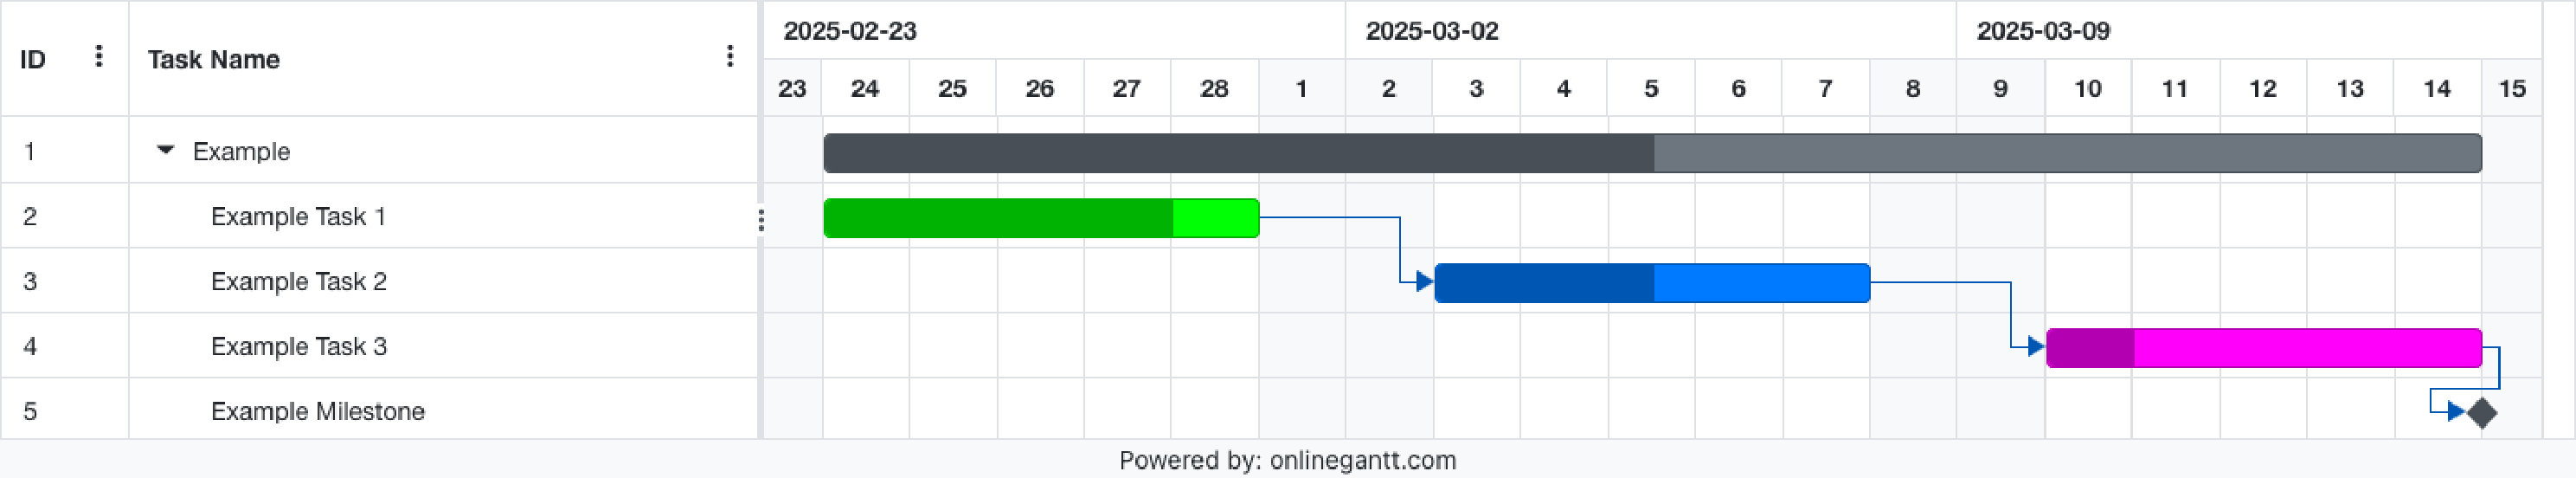
\includegraphics[width=0.8\textwidth]{images/Online Gantt 20250228.pdf}
        \hfill
    \end{figure}  
\end{frame}


% dont use this for OS, might be used for other lectures: presentation:0
\begin{frame}<presentation:0>[noframenumbering,t,plain]
\lastpage{{\usebeamerfont{title}Questions? Suggestions? Ideas?}\\[5ex]
f.n@mail.com}
\end{frame}


% ------------------------------------------------------
% backup slides
\ifincludebackup

    \begin{frame}[c]{Backup Slides ifdesired
        \begin{itemize}
            \item ...
            \item ...
        \end{itemize}
    \end{frame}    
\fi

\end{document}

